\section{Evaluation}

\begin{frame}
    \frametitle{Counting crates with UB on \texttt{crates.io} (May 2023)}
    \begin{figure}
        {\footnotesize Data obtained with the help of Ben Kimock \\
        (\href{https://github.com/saethlin/miri-tools}{github:saethlin/miri-tools})}
        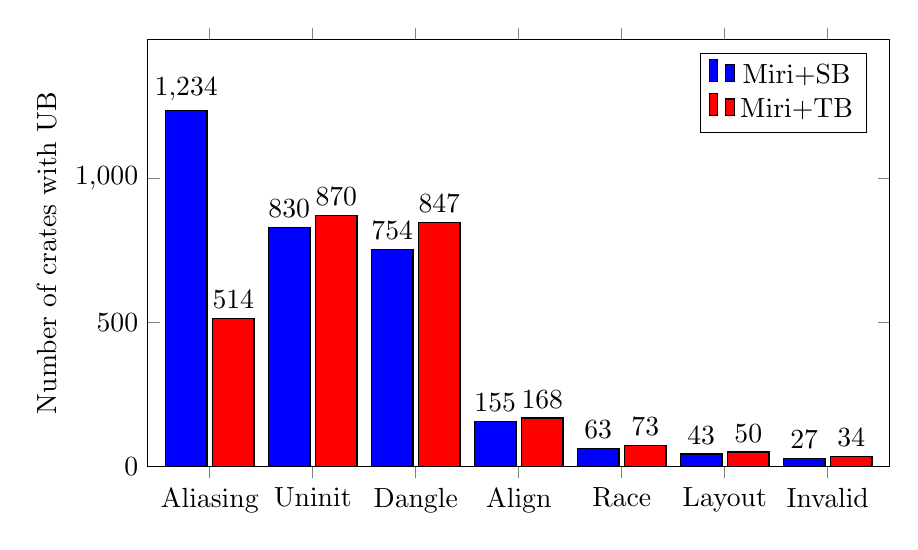
\begin{tikzpicture}
            \begin{axis}[
                    ybar,
                    ymin=0,
                    width=11cm,
                    height=7cm,
                    bar width=15pt,
                    ylabel={Number of crates with UB},
                    nodes near coords,
             %      nodes near coords align=below, % places labels inside bars
                    symbolic x coords={Aliasing, Uninit, Dangle, Align, Race, Layout, Invalid},
                    xtick = data,
                    enlarge y limits={value=0.2,upper},
                    legend pos=north east
                ]
                \addplot[fill=blue] coordinates {(Aliasing, 1234) (Uninit, 830) (Dangle, 754) (Align, 155) (Race, 63) (Layout, 43) (Invalid, 27)};
                \addplot[fill=red] coordinates {(Aliasing, 514) (Uninit, 870) (Dangle, 847) (Align, 168) (Race, 73) (Layout, 50) (Invalid, 34)};
                \legend{Miri+SB,Miri+TB}
            \end{axis}
        \end{tikzpicture}
    \end{figure}
\end{frame}

\begin{frame}
    \frametitle{Summary}
    \begin{itemize}
        \item Tree Borrows UB is much less common on \texttt{crates.io} than Stacked Borrows UB\\
            \(\qquad\Rightarrow\) fulfills goal of being more permissive
            \begin{block}{Notable examples}
                \texttt{tokio}, \texttt{pyo3}, \texttt{rkyv}, \texttt{eyre}, \texttt{ndarray},
                \texttt{arrayvec}, \texttt{slotmap}, \texttt{nalgebra}, \texttt{json}.
            \end{block}
        \item patterns allowed by Stacked Borrows but forbidden by Tree Borrows are theoretically
            possible but have not been found in actual code
    \end{itemize}
\end{frame}

\begin{frame}
    \frametitle{Reception}
    TB has existed for one year
    \begin{itemize}
        \item[$\oplus$] consensus that TB is simpler and more predictable than SB,
        \item[$\oplus$] cases where TB is more permissive than SB are welcome \\ (e.g. \texttt{\&Header} pattern),
        \item[$\oplus$] cases where TB is less permissive are rare \\ (no complaints yet),
        \item[$\ominus$] fewer optimizations (expected),
        \item[$\ominus$] controversial granularity of interior mutability,
        \item[$\ominus$] slight performance regression in Miri.
    \end{itemize}
\end{frame}

\begin{frame}
    \frametitle{Questions ?}

    Don't hesitate to test your code with Miri and send us your
    interesting/unexpected cases of UB!
    (\texttt{github:rust-lang/miri}) \\
    {\color{blue} \texttt{MIRIFLAGS=-Zmiri-tree-borrows cargo +miri miri test}}\\~\\
    \vfill

    Slides: \href{https://github.com/Vanille-N/tree-beamer/tree/etaps}{\texttt{github:Vanille-N/tree-beamer/tree/etaps}}\\
    Complementary material: \href{https://perso.crans.org/vanille/treebor}{\texttt{perso.crans.org/vanille/treebor}}\\
\end{frame}
